\documentclass[a4paper, 11pt, oneside]{book}
\usepackage{lmodern}
\usepackage[T1]{fontenc}
\usepackage[utf8]{inputenc}
\usepackage[english, italian]{babel}
\usepackage{geometry}
\usepackage{indentfirst}
\usepackage{microtype}
\usepackage{setspace}
	\onehalfspacing
\usepackage{graphicx}
\usepackage{subfig}
\usepackage{booktabs}
\usepackage{tabularx}
\usepackage{caption}
	\captionsetup{format=hang, font={small}, labelfont={bf}}
\usepackage{hyperref}
	\hypersetup{colorlinks=true, linkcolor=blue, filecolor=magenta, urlcolor=cyan,}
\usepackage{siunitx}
\usepackage{anyfontsize}
\usepackage{titlesec}
	\setcounter{secnumdepth}{3}
	\setcounter{tocdepth}{1}
\usepackage{quoting}
	\quotingsetup{font=medium}
% Pacchetti per l'inserimento di linee di codice
\usepackage{listings}
\usepackage{color}
\usepackage{xr}

\definecolor{codegreen}{rgb}{0,0.6,0}
\definecolor{codegray}{rgb}{0.5,0.5,0.5}
\definecolor{codepurple}{rgb}{0.58,0,0.82}
\definecolor{backcolour}{rgb}{1,1,1}

\lstdefinestyle{mystyle}{
    backgroundcolor=\color{backcolour},
    commentstyle=\color{codegreen},
    keywordstyle=\color{blue},
    numberstyle=\color{codegray},
    stringstyle=\color{codepurple},
    basicstyle=\footnotesize,
    breakatwhitespace=false,
    breaklines=true,
    captionpos=b,
    keepspaces=true,
    numbers=left,
    numbersep=5pt,
    showspaces=false,
    showstringspaces=false,
    showtabs=false,
    tabsize=2,
    frame=single
}

\lstset{style=mystyle}

\lstloadlanguages{C}
\lstloadlanguages{Java}

\graphicspath{{immagini/}}

\begin{document}
	\begin{titlepage}
		\begin{large}
			\begin{center}
				\LARGE{\scshape{Corso di Laurea Magistrale in \\ Computer Engineering}}\\%
				\vspace{3.0cm}%
				\LARGE{\scshape{Observe Extension of CoAP\\ with QoS}}\\%
				\vspace{4.2cm}%
				\large{Alessandro Sieni}\\%
				\large{Amedeo Pochiero}\\%
				\large{Roberto Magherini}\\%
			\end{center}
		\end{large}
	\end{titlepage}
	\frontmatter
		\tableofcontents
	\mainmatter
		\chapter{Specifiche}
L’estensione Observe del protocollo CoAP permette agli osservatori di registrarsi presso i soggetti per ottenere le risorse a cui essi sono interessati. Nel paper analizzato, è stato introdotta una funzionalità aggiuntiva che permette agli osservatori di specificare a quali eventi sono interessati, in particolare eventi critici o non critici, utilizzando dei livelli di priorità.
	\section{Processo di registrazione}
		\begin{itemize}
			\item Per inviare una registrazione l’osservatore invia una richiesta GET indicando nel campo observe il valore 0 ed un token per identificare la richiesta
			\item Nelle notifiche invece il campo observe sarà diverso da 0 ed indicherà il numero di sequenza della notifica, mantenendo invece sempre il campo token invariato
			\item Il soggetto nel momento della registrazione può decidere se rifiutare la richiesta dell’osservatore inviando la risposta priva del campo observe
			\item L’osservatore può in qualunque momento decidere di smettere di ricevere notifiche semplicemente rispondendo ad una notifica con un messaggio RST oppure inviando un messaggio GET per la stessa risorsa
			\item Per garantire l’affidabilità si fa uso dei meccanismi definiti in CoAP: un nodo che riceve un messaggio CON deve notificare che ha ricevuto correttamente il messaggio e talora il mittente non riceva un ACK, esso ritrasmetterà la richiesta. Il processo di ritrasmissione segue il modello \underline{STOP-AND-WAIT} con un backoff esponenziale
			\item Un nodo può anche scegliere di inviare messaggi in modo non affidabile usando dei messaggi NON. In questa estensione la scelta del tipo di messaggio (CON o NON) è a carico del soggetto
			\item Per la tempestività dei messaggi invece è previsto l’uso della validità temporale, avvalendosi del meccanismo di cache presente in CoAP
				\begin{itemize}
					\item In CoAP è presente un parametro MaxAge che viene usato per indicare la validità temporale
					\item Un osservatore può salvare in cache un messaggio e riutilizzarlo per future richieste finché la sua validità temporale sarà rispettata
				\end{itemize}
		\end{itemize}

	\section{Ruoli}
		\subsection{Subject}
			Non gestisce le code a priorità. Effettua un sensing costante in modo da non perdersi gli eventi critici. I dati collezionati vengono inviati solamente al proxy e non direttamente agli osservatori.
		\subsection{Proxy CoAP-CoAP}
			Gestisce le code a varie priorità. Riceve le richieste di registrazione alle risorse da parte degli osservatori, quindi registra sé stesso presso i soggetti per ricevere le notifiche di quelle risorse. In questo modo, si maschera anche il numero di osservatori interessati alla risorsa e si riduce il numero di pacchetti inviati dai soggetti, in quanto questi manderanno solo al proxy, il quale appare come un unico osservatore. 
		\subsection{Border Router}
			Si occupa di fare da tramite tra la rete locale dei nodi sensori e il proxy.
		\subsection{Observer}
			Richiede al proxy la lista delle risorse disponibili sui vari soggetti ed effettua una registrazione per ogni risorsa a cui è interessato. Se la notifica della risorsa non viene ricevuta entro il MaxAge dell’ultimo pacchetto ricevuto, l’osservatore considera sé stesso eliminato dalla lista di osservatori da notificare. 

	\section{Gestione della Frequenza di trasmissione}
		Al fine di limitare il numero di trasmissioni effettuate dai nodi sensori, e quindi di ridurre il consumo della batteria degli stessi, la frequenza di trasmissione dei nodi sensori al proxy varia nel tempo in base ai valori che stanno rilevando. Nel caso in cui i valori si mantengono per un periodo di tempo all’interno di una certa fascia non critica, la frequenza di trasmissione può essere abbassata, fino a raggiungere un valore minimo prefissato. Viceversa, alla rilevazione di un evento critico, la frequenza di trasmissione è aumentata, quindi successivamente, quando i valori non sono considerati più critici si ripete l’algoritmo per trovare il numero minimo di trasmissioni necessarie. Per implementare questo meccanismo si sfrutta il campo MaxAge del protocollo CoAP, in modo tale da far sapere all’osservatore per quanto tempo deve essere considerato valido il valore ricevuto, in quanto se non riceve alcun nuovo valore entro il MaxAge dell’ultimo pacchetto ricevuto, l’osservatore si può considerare eliminato dalla lista degli osservatori gestiti da tale soggetto.
		\chapter{Modulo ProxyObserver}
	\section {Descrizione}
	\section {Implementazione}
		\subsection {Modifiche a Californium lato Server}
			Al fine di implementare le modifiche effettuate al protocollo CoAP, è stato necessario modificare anche la libreria Californium. In seguito verranno elencati i cambiamenti al codice della libreria, indicando il nome del file con un link alla repository con il codice originale e la motivazione di tale modifica. I file fanno riferimento alla package core di Californium:
			\subsubsection{coap.CoAP}
				Il livello di priorità viene indicato usando i primi 2 bit, rinominato campo \textit{QoS} del campo Observe del pacchetto CoAP ( 3 bytes ).  Questa classe fornisce i valori che questo campo può assumere\newline
				\lstinputlisting[language=Java, firstline=663, lastline=673, caption={coap.CoAP.QoSLevel, \href{https://tinyurl.com/y46rbbg6}{codice originale}},captionpos=b]{../Codice/Java/CoAP.java}

			\subsubsection{coap.Request}
				Nel protocollo standard una Observe Request Registration può avere solo il valore 0 nel campo \textit{Observe}. Nel caso considerato invece i valori possono essere 4, corrispondenti ai 4 livelli di priorità. Questa funzione deve ritorna \textit{True} se 	contiene uno di questi valori. \newline
				\lstinputlisting[language=Java, firstline=636, lastline=643, caption={coap.Request, \href{https://tinyurl.com/y2lhtgo4}{codice originale} },captionpos=b]{../Codice/Java/Request.java}

			\subsubsection{observe.ObserveRelation}
			Una ObserveRelation mantiene le informazioni relative alla relazione tra un observer e la risorsa osservata. \'E stato aggiunto un 	campo alla classe per mantenere il livello di priorità di quella relazione, i suoi get e set e una funzione per comparare 2 relazioni in base a questo campo. Quest'ultima servirà nel meccanismo di notifica degli observer basato su priorità. \newline
				\lstinputlisting[language=Java, firstline=61, lastline=63, caption={observe.ObserveRelation QoS, \href{https://tinyurl.com/y3rf5qgl}{codice originale}},captionpos=b]{../Codice/Java/ObserveRelation.java}
				\lstinputlisting[language=Java, firstline=130, lastline=147, caption={observe.ObserveRelation funzioni QoS, \href{https://tinyurl.com/y3rf5qgl}{codice originale}},captionpos=b]{../Codice/Java/ObserveRelation.java}

			\subsubsection{server.ServerMessageDeliverer}
				Quando una \textit{ObserveRelation} viene creata in seguito alla ricezione di una richiesta con l’opzione Observe, il campo \textit{QoS} della relazione viene settato con il valore del campo Observe della richiesta. \newline
				\lstinputlisting[language=Java, firstline=153, lastline=165, caption={server.ServerMessageDeliverer checkForObserveOption(...), \href{https://tinyurl.com/y3tom2xy}{codice originale}},captionpos=b]{../Codice/Java/ServerMessageDeliverer.java}

			\subsubsection{server.ServerState}
				Enumerato che definisce i 3 stati del nodo sensore:
				\begin{enumerate}
					\item \textbf{UNAVAILABLE}: il nodo sensore non è attivo, qualsiasi richiesta relativa a quel sensore è rigettata.
					\item \textbf{ONLY\_CRITICAL}: il nodo sensore ha un autonomia al di sotto di una certa soglia, quindi si accettano solo richieste da parte di observe richiedenti solo gli eventi critici della risorsa.
					\item \textbf{AVAILABLE}: il nodo non ha problemi di autonomia quindi è possibile accettare qualsiasi tipo di richiesta.
				\end{enumerate}
				\lstinputlisting[language=Java, firstline=3, lastline=5, caption={ServerState},captionpos=b]{../Codice/Java/ServerState.java}

			\subsubsection{CoapResource}
				\paragraph{Aggiornamento relazioni dopo il cambio stato del sensore}
				Quando avviene un cambio di stato di un sensore, è necessario controllare che le relazioni già stabilite siano consistenti con il nuovo stato. Pertanto quando lo stato diventa \textbf{ONLY\_CRITICAL}, le relazioni con livello \textit{CoAP.QoSLevel.NON\_CRITICAL\_MEDIUM\_PRIORITY} e \textit{CoAP.QoSLevel.NON\_CRITICAL\_LOW\_PRIORITY} vengono cancellate, mentre se si passa ad \textbf{UNAVAILABLE}, tutte le relazioni di quella risorsa vengono cancellate. \'E stata quindi aggiunta una funzione per cancellare solo le relazioni con un livello non critico di priorità. \newline
				\lstinputlisting[language=Java, firstline=557, lastline=567, caption={CoapResource clearAndNotifyNonCriticalObserveRelations, \href{https://tinyurl.com/y264lheh}{codice originale}},captionpos=b]{../Codice/Java/CoapResource.java}
				\paragraph{Notifica basata su priorità}
				È stata aggiunta una lista \textit{sortedObservers} di ObserveRelation ordinata in base al campo \textit{QoS} di un ObserveRelation in modo decrescente. L’ordinamento è effettuato all’inserimento di una nuova relazione nel \textit{ObserveRelationContainer observeRelations}. Questa nuova lista è impiegata per effettuare l’invio delle notifiche in ordine di priorità: l'invio delle notifiche è effettuato scansionando in modo sequenziale questa lista, partendo dal primo elemento ( priorità maggiore ), fino all'ultimo elemento ( priorità minore ). Per mantenere la lista consistente con l’ObserveRelationContainer, alla rimozione di un elemento da quest’ultimo, si rimuove lo stesso dalla sortedObservers.\newline
				\lstinputlisting[language=Java, firstline=176, lastline=179, caption={CoapResource sortedObservers, \href{https://tinyurl.com/y264lheh}{codice originale}},captionpos=b]{../Codice/Java/CoapResource.java}
				\lstinputlisting[language=Java, firstline=809, lastline=831, caption={CoapResource addObserveRelation(...), \href{https://tinyurl.com/y264lheh}{codice originale}},captionpos=b]{../Codice/Java/CoapResource.java}
				\lstinputlisting[language=Java, firstline=840, lastline=852, caption={CoapResource removeObserveRelation(...), \href{https://tinyurl.com/y264lheh}{codice originale}},captionpos=b]{../Codice/Java/CoapResource.java}
				\lstinputlisting[language=Java, firstline=915, lastline=925, caption={CoapResource notifyObserverRelations(...), \href{https://tinyurl.com/y264lheh}{codice originale}},captionpos=b]{../Codice/Java/CoapResource.java}

		\chapter{Modulo ProxySubject}
\section{Descrizione}
Questo modulo permette la gestione della comunicazione tra il \textbf{Proxy} e i \textbf{Subjects} fornendo le informazioni necessarie al modulo \textbf{ProxyObserver}.\\
Le informazioni che dovranno essere mantenute da questo modulo sono tutte quelle necessarie ad evitare comunicazioni non necessarie tra gli osservatori ed i soggetti, in quanto dovrà essere proprio il modulo \textbf{ProxySubject} ad offire le informazioni richieste, qualora sia possibile. \\
In particolare il modulo si occuperà di gestire una struttura dati che dovrà rappresentare il soggeto dal punto di vista dell'osservatore, offrendo informazioni quali lo stato del soggetto (ovvero quali tipologie di richieste è in grado di accettare), le risorse offerte dal soggetto, in modo tale da non dover sprecare tempo ed energia per richiedere ogni volta se può o meno offrire una determinata risorsa, sulla quale il soggetto ha già ricevuto una registrazione, in quanto se un osservatore vuole effettuare una registrazione al proxy su una risorsa a cui un altro osservatore ha fatto la medesima richiesta, con le stesse caratteristiche in termini di priorità, allora quest'ultima non sarà inoltrata al soggetto in quanto il proxy è in grado di poterla gestire in completa autonomia. \\
In aggiunta il modulo  \textbf{ProxySubject} offre anche un meccanismo di cache dei valori ricevuti, in modo tale da memorizzare l'ultimo valore ottenuto da un soggetto in una struttura dati, utile al modulo \textbf{ProxyObserver} qualora dovesse richiedere un valore ad un determinato soggetto, come ad esempio durante la fase di registrazione.
\section{Implementazione}
\subsection{CacheTable}
Questa classe si occupa di mantenere le informazioni ottenute dai soggetti e di renderle disponibili in qualunque momento.
\subsubsection{Inserimento Valori}
Quando viene ricevuto un nuovo valore dai soggetti è necessario inserire il valore nella cache, controllando se era già stato ricevuto un valore relativo a quella registrazione, in tal caso aggiornando il vecchio valore, oppure se inserire un nuovo valore, in quanto quello appena ricevuto risulta essere il primo valore ricevuto relativo alla registrazione associata ad esso. \\
\lstinputlisting[language=Java,firstnumber=28, firstline=28, lastline=40, caption={CacheTable.InsertData}]{../Codice/Java/ProxySubject/CacheTable.java}
\subsubsection{Aggiornamento dei valori}
Per mantenere consistenti i valori presenti in cache è opportuno che questi ultimi siano periodicamente aggiornati - abbiamo scelto una frequenza di aggiornamento di 1Hz - in quanto uno degli elementi su cui si basa l'intero protocollo è il valore MaxAge appartenente ad ogni singolo valore, in quanto nel momento in cui tale valore raggiunge lo 0 e non si è ricevuto alcun valore successivo, allora si deve considerare terminato l'ascolto verso il soggetto,e non aspettarsi più alcun valore. \\
\lstinputlisting[language=Java,firstnumber=14, firstline=14, lastline=27, caption={CacheTable.updateTime}]{../Codice/Java/ProxySubject/CacheTable.java}
\subsection{Gestione delle notifiche}
Per gestire le notifiche da parte dei soggetti abbiamo continuato ad appoggiarci a Californium, in particolare definendo una classe ResponseHandler come estenesione della CoAPHandler, in quanto erano necessarie alcune operazioni da effettuare subito dopo la ricezione del messaggio. \\
In particolare la prima operazione da eseguire è quella di discriminare se il messaggio appena ricevuto è critico o meno, risultato ottenuto analizzando il contenuto del messaggio, in quanto la politica di valutazione di un valore è implementata nei soggetti ed ignota al proxy. Questo significa che se al termine del valore è presente il carattere '!' allora significa che il valore ricevuto deve essere gestito come valore critico, altrimenti risulta essere un valore non critico. \\
Discriminato il valore dovrà essere creato un nuovo \textbf{SensorData}, che rappresenta in tutti gli aspetti il valore appena ricevuto, e che dovrà essere inserito in cache. Solo al termine di quest'ultima operazione dovrà esssre informato il modulo \textbf{ProxyObserver} in modo che notifichi il nuovo valore a tutti gli osservatori registrati per tale risorsa. \\
In seguito è riportato solo una parte del codice per la gestione del messaggio, ovvero solo quella ritenuta interessante. \\
\lstinputlisting[language=Java,firstnumber=41, firstline=41, lastline=72, caption={Parte del metodo ResponseHandler.onLoad}]{../Codice/Java/ProxySubject/ResponseHandler.java}
\subsection{Registrator}
Questa classe serve a gestire il processo di registrazione, in particolare analizza se quest'ultima risulta essere necessaria oppure se la vecchia registrazione debba essere aggiornata. \\
\subsubsection{Inserimento di una nuova registrazione}
Una volta ricevuta una richiesta di registrazione da parte di un osservatore è necessario verificare se tale registrazione è necessaria o meno, ed eventualmente portarla a termine mediante il metodo messo a disposizione dalla classe \textbf{Registration}. \\
Per controllare se a seguito della richiesta di registrazione ricevuta dal proxy, è necessario inoltrarla al soggetto interessato o se invece le registrazioni già presenti riescono a coprire anche la nuova richiesta, evitando quindi spreco di tempo ed energia da parte del soggetto; è necessario analizzare il soggetto relativo a tale registrazione, la risorsa richiesta e il livello di criticità desiderato: se è già presente una registrazione avente lo stesso soggetto, associata alla stessa risorsa e con un livello di criticità minore rispetto a quello richiesto - in quanto se per esempio venisse fatta una richiesta solo per valori critici ma ce ne fosse una che li copre tutti, allora non sarebbe necessaria adempiere alla richiesta appena arrivata - allora il processo di registrazione verrbbe completato senza consultare il soggetto, in quanto per quest'ultimo non cambierebbe niente. In alternativa se è presente una registrazione con un livello maggiore rispetto a quello richiesto - si prenda ad esempio il caso opposto rispetto a quello illustrato prima - la vecchia registrazione non sarà sufficiente e quindi dovrà essere aggiornata in modo da coprire anche la richiesta appena arrivata. \\
\lstinputlisting[language=Java,firstnumber=13, firstline=13, lastline=59,caption={Registrator.newRegistration e Registrator.RegistrationNeeded}]{../Codice/Java/ProxySubject/Registrator.java}
\subsubsection{Rimozione di una registrazione}
Qualora non si ricevessere più notifiche da parte del soggetto o se tutti gli osservatori - in quanto basta almeno un osservatore interessato per mantenere attiva la registrazione - non desiderassero ricevere più notifiche, risulta necessario rimuovere la registrazione e notificare al soggeto che non siamo più registrati per tale risorsa. \\
\lstinputlisting[language=Java,firstnumber=69, firstline=69, lastline=81,caption={Registrator.removeRegistration}]{../Codice/Java/ProxySubject/Registrator.java}
\subsection{Virtualizzare soggetti e messaggi}
Un aspetto molto importante del modulo \textbf{ProxySubject} è la capacità di virtualizzare sia i soggetti che i messaggi ricevuti da essi, in modo da rendere completamente trasparente il comportamento dei nodi sensori per il modulo \textbf{ProxyObserver} e quindi di conseguenza per gli osservatori. \\
Tale scelta di sviluppo ha comportato la possibilità di sviluppare in modo indipendente i protocolli di comunicazione con gli osservatori da una parte e con i soggetti dall'altra, in quanto l'unica cosa a comune risultano essere proprio le strutture dati che \textit{virtualizzano} i soggetti e i messaggi ricevuti da essi.
\subsubsection{SensorNode}
Questa classe si occupa di gestire un soggetto, mantenendo le informazioni necessarie, il suo URI, le risorse che mette a disposizione, il suo livello di batteria e lo stato in cui opera, che può essere:
\begin{itemize}
  \item \textbf{UNAVAILABLE}: Il sensore non è raggiungibile in quanto le batterie sono scariche.
  \item \textbf{ONLYCRITICAL}: Il livello di batteria è troppo basso quindi il soggetto accetta solo registrazioni critiche.
  \item \textbf{AVAILABLE}: Il livello di batteria è sufficientemente alto per gestire qualsiasi tipo di registrazione
\end{itemize}
\lstinputlisting[language=Java,firstnumber=12, firstline=12, lastline=16,caption={Attributi offerti e gestiti dalla clase SensorNode}]{../Codice/Java/ProxySubject/SensorNode.java}
In particolare per la gestione della batteria è stato scelto di adottare un approccio che prevede l'invio di nuovi aggiornamenti da parte del soggetto solo qualora il livello della batteria sia inferiore alla soglia critica, in modo da ridurre il numero di messaggi inviati dal soggetto stesso, prolungando la durata della sua batteria. Ricevuto il valore poi sarà carico del proxy aggiornare lo stato del soggetto \textit{virtuale} in modo che sia consistente con lo stato del relativo soggetto reale. \\
\lstinputlisting[language=Java,firstnumber=42, firstline=42, lastline=59,caption={SensorNode.UpdateBattery}]{../Codice/Java/ProxySubject/SensorNode.java}
\subsubsection{SensorData}
Questa classe si occupa invece di gestire e rendere facilmente accessibili i messaggi ottenuti dai soggetti, con le relative informazioni di contorno, come il soggetto mittente, la registrazione a cui quel valore è associato, il maxage del messaggio e se è o meno un messaggio critico. \\
\lstinputlisting[language=Java,firstnumber=7, firstline=7, lastline=11,caption={Attributi gestiti e offerti dalla classe SensorData}]{../Codice/Java/ProxySubject/SensorData.java}

		\chapter{Observer}
	\section {Descrizione}
		Questo programma permette di usare un CoapClient e interagire con i sensori tramite il Proxy tramite una shell che dispone dei seguenti comandi:
		\begin{enumerate}
			\item Stampa il menu di aiuto
			\item Richiedi una registrazione selezionando tra quelle disponibili, specificando la priorità e la volontà ad accettare una eventuale proposta del sensore durante la negoziazione
			\item Richiedi la cancellazione di una relazione
			\item Avvia la discovery delle risorse
		\end{enumerate}
	\section {Implementazione}
		\subsection {Modifiche a Californium lato Client}
			Al fine di implementare le modifiche effettuate al protocollo CoAP, è stato necessario modificare anche la libreria Californium. In seguito verranno elencati i cambiamenti al codice della libreria, indicando il nome del file con un link alla repository con il codice originale e la motivazione di tale modifica. I file fanno riferimento alla package core di Californium:
			\subsubsection{CoapClient}
				Con l'introduzione della negoziazione del livello di priorità è necessario effettuare ulteriori controlli alla risposta ricevuta. Nel caso in cui la negoziazione è stata avviata, la risposta avrà come \textit{ResponseCode} \textbf{NOT\_ACCEPTABLE} e la CoapObserveRelation appena creata viene cancellata. Se la registrazione viene accettata senza negoziazione, allora bisogna controllare che il campo \textit{Observe} della risposta coincida con quello della richiesta. In ogni caso, dopo la ricezione della risposta, l'ordine delle notifiche deve essere resettato, in quanto la risposta alla registrazione può contenere nel campo Observe il valore della priorità, il quale può essere maggiore dell'attuale numero di notifica (vedere meccanismo di riordinamento delle notifiche.\newline
				\lstinputlisting[label={observeAndWaitNegotiation}, language=Java, firstline=1148, lastline=1177, caption={CoapClient, \href{https://tinyurl.com/y25fegl8}{codice originale}},captionpos=b]{../Codice/Java/CoapClient.java}
			\subsubsection{CoapObserveRelation}
				Per resettare il gestore dell'ordine delle notifiche, è sufficiente ridefinire l'oggetto.\newline
				\lstinputlisting[language=Java, firstline=286, lastline=290, caption={CoapObserveRelation, \href{https://tinyurl.com/y4ockh22}{codice originale}},captionpos=b]{../Codice/Java/CoapObserveRelation.java}
		\subsection{classe Observer}
			Questa classe utilizza un \textit{CoapClient} per effettuare le richeste verso il Proxy. Inoltre, mantiene le informazioni relative alle risorse trovate durante la discovery e una lista delle relazioni attualmente attive.
			\subsubsection{resourceRegistration}
				Prepara una richiesta di tipo \textbf{GET} contenente nel campo \textit{Observe} il valore specificato dall'utente e la invia utilizzando la funzione \ref{observeAndWaitNegotiation}

		\chapter{Subject}
  \section{Descrizione}
    Questo è il firmware che verrà eseguito sui \textit{nodi sensore}, i quali si comporteranno come dei CoapServer, avviando un server rest, in ascolto sulla porta di default
    di CoAP 5683, gestendo le richieste ricevute dal \textit{Proxy}, che possono essere:
    \begin{itemize}
      \item Discovery delle risorse presenti sul nodo
      \item Registrazione ad una risorsa con uno specifico tipo di priorità
      \item Cancellazione dall'osservazione di una risorsa
    \end{itemize}
    Il nodo sensore, solo nel caso in cui è registrato almeno un \textit{Observer} ad una risorsa, si occuperà di eseguire il sensing e l'invio di quest'ultima nel caso in cui
    il valore sia cambiato o il vecchio valore stia per scadere (questo secondo caso è gestito per evitare di perdere la registrazione dell'\textit{Osservatore}).\newline
    Il nodo sensore si occupa anche di connettersi e di mantenere viva la connessione col \textit{Border Router}, utilizzato dal \textit{Proxy} per comunicare con i nodi sensore.

  \section{Modifiche al Border Router}
    Per poter compilare il codice del border router fornito con contikiOS per dispositivi di tipo SkyMote è stato necessario disabilitare il processo che esegue il web server in quanto il dispositivo non dispone di
    memoria sufficiente per poter utilizzare questa funzione; la quale veniva utilizzata semplicemente con lo scopo di far vedere all'utente le rotte presenti al momento e la lista dei vicini tramite interfaccia web,
    quindi rimuovendo questo processo non vengono rimosse funzionalità necessarie ad un router.\newline
    Per rimuovere la funzionalità è bastato ridefinire WEBSERVER uguale a 0.
    \lstinputlisting[label={BorderRouter}, language=C, firstnumber=64 ,firstline=64, lastline=67, caption={BorderRouter, \href{https://tinyurl.com/yxzcal2z}{codice originale}},captionpos=b]{../Codice/C/border-router.c}

  \section{Implementazione}
    \subsection{Process Rest Server}
      Processo principale dei nodi sensore, si occupa di:
      \begin{enumerate}
        \item Ottenere un indirizzo IP connettendosi al border-router
        \item Rendere disponibili le risorse presenti attivandole
        \item Attivare i sensori relativi alle singole risorse
      \end{enumerate}

      %A seconda di come viene usato e se viene usato o meno alla fine del progetto, inserisci qualche nota relativa a powertrace

      \lstinputlisting[label={RestServer}, language=C, firstnumber=38, firstline=38, caption={Process RestServer},captionpos=b]{../Codice/C/subscriber.c}

    \subsection{Risorse}
      Per avere una maggiore modularità è stato realizzato un file per ogni singola risorsa e risorse sono state definite come variabili di tipo \textbf{extern}

      \lstinputlisting[label={ExternResources}, language=C, firstnumber=4, firstline=4, lastline=12, caption={Risorse presenti sul nodo},captionpos=b]{../Codice/C/subscriber.c}

      Per il nostro scopo vengono utilizzate esclusivamente risorse osservabili, che devono essere dichiarate come risorse di tipo \textbf{PERIODIC\_RESOURCE};
      la peculiarità di questo tipo di risorse è il fatto che al momento dell'inizializzazione sono necessarie, tra le altre cose:
      \begin{itemize}
        \item get\_handler: una funzione utilizzata nel caso in cui venga fatta una richiesta di tipo get alla risorsa (necessaria anche per risorse non periodiche),
              ma che viene richiamata, anche, ogni volta sia necessario inviare un nuovo valore ai vari osservatori
        \item Il periodo con il quale viene richiamata la funzione periodic\_handler
        \item periodic\_handler: una funzione che viene utilizzata per eseguire il sensing della risorsa, verificare se è necessario o meno inviare il valore ottenuto, a causa
              della scandenza della vecchia risorsa oppure della rilevazione di un valore critico o meno che differisce dal precedente di una certa soglia, e in caso di invio
              decide anche il valore del campo MaxAge
      \end{itemize}

      \subsubsection{Batteria}
        La batteria viene fornita come risorsa di tipo osservabile, l'unico osservatore che si iscrive per ricevere le notifiche relative a questa risorsa è il \textit{Proxy},
        in quanto se la batteria del sensore si trova sotto una specifica soglia (\textbf{CRITICAL\_BATTERY}) vengono accettate
        soltanto richieste con un livello di priorità critico.\newline
        Il livello della batteria è simulato e viene fatto variare in base al tipo di operazione (sensing e trasmissione del valore)
        di una certa quantità costante differente per ogni tipologia (\textbf{SENSING\_DRAIN}, \textbf{TRANSMITTING\_DRAIN}).\newline
        Il sensing del livello della batteria viene fatto periodicamente.Invece per quanto riguarda le notifiche della batteria vengono inviate solo in due casi:
        \begin{enumerate}
          \item Valore della batteria è sotto la soglia critica
          \item L'ultimo valore sta per scadere, per evitare che il protocollo per la registrazione alla batteria venga rieseguito nuovamente
        \end{enumerate}

        Una volta che la batteria è stata inviata perché la soglia è scesa sotto il livello critico, questa non verrà più inviata al \textit{Proxy} in quanto ormai gestisce le richieste di registrazione in modo
        opportuno e sa che dal momento in cui non riceverà più valori da quel nodo, questo non avrà più batteria.

        \lstinputlisting[label={res-battery}, language=C, caption={Codice di gestione relativo alla risorsa batteria},captionpos=b]{../Codice/C/resources/res-battery.c}


      \subsubsection{Temperatura}

    \subsection{Parametri}

		\externaldocument{ProxyObserver.tex}
\chapter{Testing}
  I testing delle modifiche effettuate al Procotollo CoAP sono stati effettuati utilizzando i seguenti dispositivi:
  \begin{itemize}
    \item x2 Zolertia Z1 mote sui quali viene eseguito il codice relativo al Subject
    \item Tmote Sky usato come border router che permette di accedere alla rete locale dei Subject
    \item Raspberry Pi 3 Model B che interpreta il Proxy
    \item Una macchina in grado di eseguire il codice dell'Observer
  \end{itemize}
  L'architettura finale risulta quindi essere la seguente \ref{fig:architettura}
  \begin{figure}
    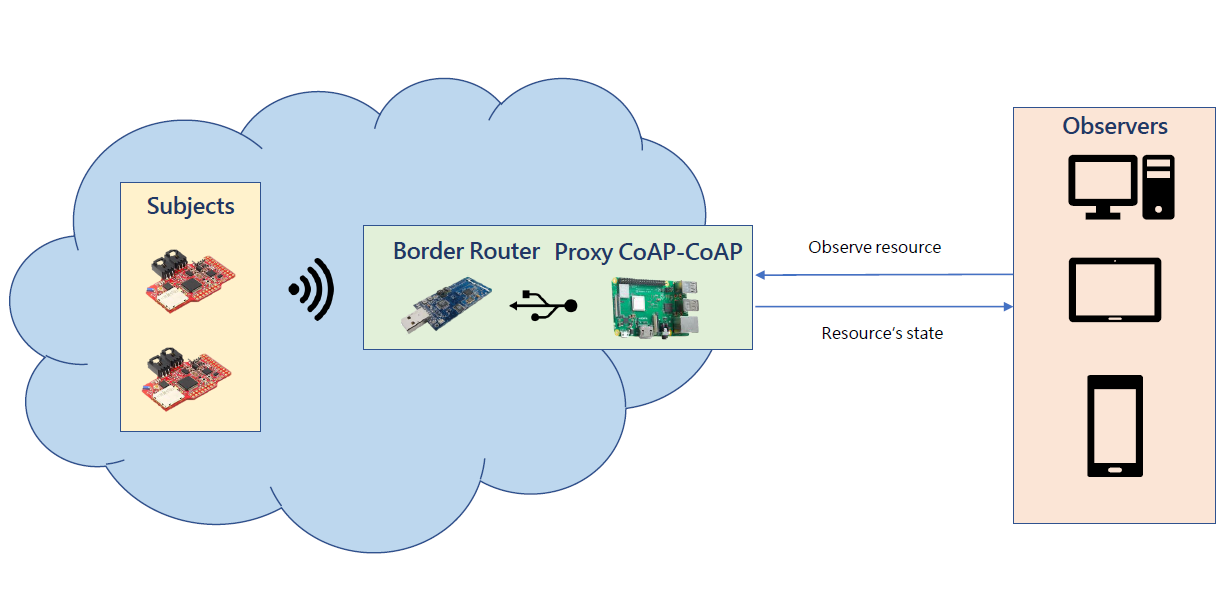
\includegraphics[width=\linewidth]{../Immagini/ArchitetturaGenerale.png}
    \caption{Ambiente di Testing}
    \label{fig:architettura}
  \end{figure}
  \section{Ritardo Trasmissione}
    Seguendo il meccanismo di tramissione spiegato in \ref{NotificaPriotita}, il \textit{ProxyObserver} invia le notifiche in modo ordinato agli osservatori, nel seguente ordine:
    \begin{enumerate}
      \item \textbf{CoAP.QoSLevel.CRITICAL\_HIGHEST\_PRIORITY}
      \item \textbf{CoAP.QoSLevel.CRITICAL\_HIGH\_PRIORITY}
      \item \textbf{CoAP.QoSLevel.NON\_CRITICAL\_MEDIUM\_PRIORITY}
      \item \textbf{CoAP.QoSLevel.NON\_CRITICAL\_LOW\_PRIORITY}
    \end{enumerate}
    Questo si riflette sul tempo necessario ad un osservatore a ricevere la propria notifica, in particolare gli osservatori registrati sulla stessa risorsa dello stesso sensore, riceveranno le notifiche in istanti diversi dipendentemente dal loro livello di priorità.
    Il testing effettuato permette di evidenziare questa conseguenza del nuovo meccanismo di invio e si basa sull'acquisizione del timestamp in 2 istanti precisi:
    \begin{enumerate}
      \item Istante di \textbf{invio} della notifica da parte del \textit{Subject}
      \item Istante di \textbf{ricezione} della notifica da parte del \textit{Observer}
    \end{enumerate}
    Sono stati avviati 16 Observer, in particolare 4 Observer per ogni priorità. Questi hanno richiesto al Proxy le notifiche della temperatura di un sensore, simulando che quest'ultimo sia costantemente in una situazione di criticità, in modo che tutti gli observer ricevino lo stesso numero di notifiche. \newline
    L'esecuzione è proseguita per un certo intervallo di tempo in cui sono state ricevute circa 40 notifiche, per ognuno delle quali sono stati salvati i timestamp di ricezione in un log relativo ad ogni observer, oltre al log del Subject in cui sono stati salvati i timestamp di invio. A questo punto, è stato possibile analizzare i file creati tramite uno script Python che calcola il ritardo di trasmissione medio dei pacchetti per ogni priorità. \newline
    I risultati ottenuti variano in base all'ambiente in cui sono stati effettuati i testing, in particolare:
    \begin{itemize}
      \item Canale di comunicazione con poche interferenze \ref{fig:graficoRitardoLibero}
      \item Canale di comunicazione abbastanza disturbato \ref{fig:graficoRitardoDisturbato}
    \end{itemize}
    In entrambi è evidente come all'aumentare della priorità il ritardo medio si riduce.
    \begin{figure}
      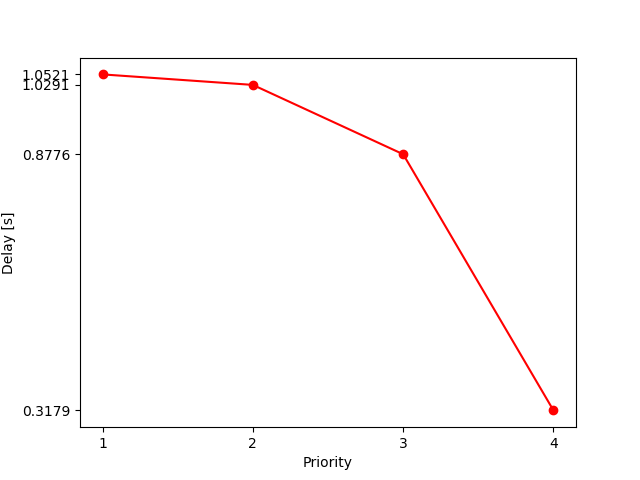
\includegraphics[width=\linewidth]{../Immagini/GraficoRitardoLibero.png}
      \caption{Grafico del ritardo al variare della priorità degli Observer con canale libero}
      \label{fig:graficoRitardoLibero}
    \end{figure}
    \begin{figure}
      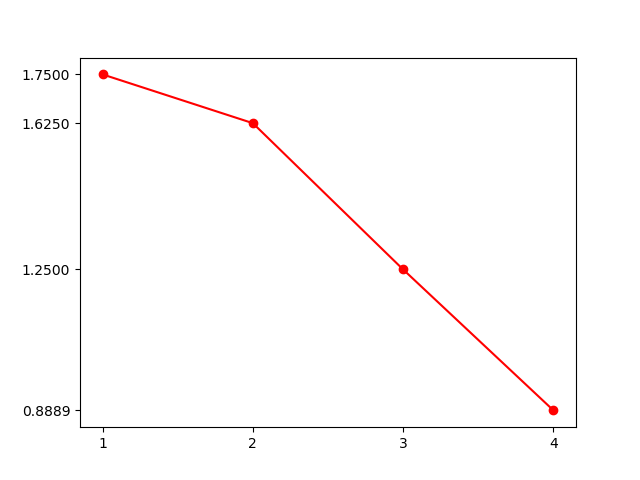
\includegraphics[width=\linewidth]{../Immagini/GraficoRitardoDisturbato.png}
      \caption{Grafico del ritardo al variare della priorità degli Observer con canale disturbato}
      \label{fig:graficoRitardoDisturbato}
    \end{figure}

\end{document}
